% diagram-kind: memory
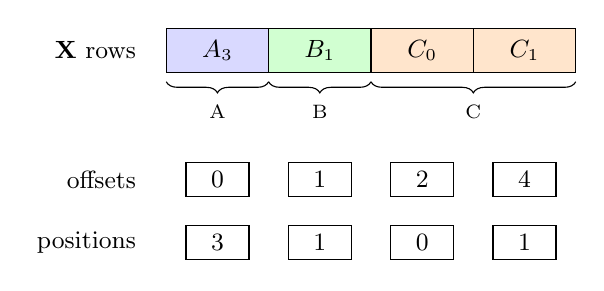
\begin{tikzpicture}[font=\small,x=1.3cm,y=.8cm]
\node[anchor=east] at (-.2,3.6) {$\mathbf X$ rows};
\foreach \x/\lab/\fillc in {0/$A_3$/blue!15,1/$B_1$/green!18,2/$C_0$/orange!20,3/$C_1$/orange!20} {
  \draw[fill=\fillc] (\x,3.25) rectangle ++(1,.7);
  \node at (\x+.5,3.6) {\lab};
}
\node[anchor=east] at (-.2,1.55) {offsets};
\foreach \x/\lab in {0/0,1/1,2/2,3/4} {
  \node[draw,minimum width=.8cm] at (\x+.5,1.55) {\lab};
}
\node[anchor=east] at (-.2,.55) {positions};
\foreach \x/\lab in {0/3,1/1,2/0,3/1} {
  \node[draw,minimum width=.8cm] at (\x+.5,.55) {\lab};
}
\draw[decorate,decoration={brace,mirror,amplitude=4pt}] (0,3.1)--(1,3.1)
 node[midway,below=5pt,font=\scriptsize]{A};
\draw[decorate,decoration={brace,mirror,amplitude=4pt}] (1,3.1)--(2,3.1)
 node[midway,below=5pt,font=\scriptsize]{B};
\draw[decorate,decoration={brace,mirror,amplitude=4pt}] (2,3.1)--(4,3.1)
 node[midway,below=5pt,font=\scriptsize]{C};
\end{tikzpicture}
